
\documentclass[10pt, conference, compsocconf]{IEEEtran}

% Add the compsocconf option for Computer Society conferences.
%
% If IEEEtran.cls has not been installed into the LaTeX system files,
% manually specify the path to it like:
% \documentclass[conference]{../sty/IEEEtran}


\usepackage{balance}
\usepackage{amssymb}
\setcounter{tocdepth}{3}
\usepackage{graphicx}
 
\usepackage{url}





% *** GRAPHICS RELATED PACKAGES ***
%
\ifCLASSINFOpdf
  % \usepackage[pdftex]{graphicx}
  % declare the path(s) where your graphic files are
  % \graphicspath{{../pdf/}{../jpeg/}}
  % and their extensions so you won't have to specify these with
  % every instance of \includegraphics
  % \DeclareGraphicsExtensions{.pdf,.jpeg,.png}
\else
  % or other class option (dvipsone, dvipdf, if not using dvips). graphicx
  % will default to the driver specified in the system graphics.cfg if no
  % driver is specified.
  % \usepackage[dvips]{graphicx}
  % declare the path(s) where your graphic files are
  % \graphicspath{{../eps/}}
  % and their extensions so you won't have to specify these with
  % every instance of \includegraphics
  % \DeclareGraphicsExtensions{.eps}
\fi
% graphicx was written by David Carlisle and Sebastian Rahtz. It is
% required if you want graphics, photos, etc. graphicx.sty is already
% installed on most LaTeX systems. The latest version and documentation can
% be obtained at: 
% http://www.ctan.org/tex-archive/macros/latex/required/graphics/
% Another good source of documentation is "Using Imported Graphics in
% LaTeX2e" by Keith Reckdahl which can be found as epslatex.ps or
% epslatex.pdf at: http://www.ctan.org/tex-archive/info/
%
% latex, and pdflatex in dvi mode, support graphics in encapsulated
% postscript (.eps) format. pdflatex in pdf mode supports graphics
% in .pdf, .jpeg, .png and .mps (metapost) formats. Users should ensure
% that all non-photo figures use a vector format (.eps, .pdf, .mps) and
% not a bitmapped formats (.jpeg, .png). IEEE frowns on bitmapped formats
% which can result in "jaggedy"/blurry rendering of lines and letters as
% well as large increases in file sizes.
%
% You can find documentation about the pdfTeX application at:
% http://www.tug.org/applications/pdftex




% correct bad hyphenation here
\hyphenation{op-tical net-works semi-conduc-tor}


\begin{document}
%
% paper title
% can use linebreaks \\ within to get better formatting as desired
\title{Handling Contract Violations in Java Card Using Explict Exception Channels}


% author names and affiliations
% use a multiple column layout for up to two different
% affiliations

\author{\IEEEauthorblockN{Juliana Ara\'ujo, Rafael Souza, N\'elio Cacho,
Anamaria Moreira} 
\IEEEauthorblockA{Computing and Applied Mathematics Department (DIMAp)\\ 
Federal University of Rio Grande do Norte (UFRN)\\
 Natal-RN, Brazil\\
 \{juliana,rafael,neliocacho,anamaria\}@dimap.ufrn.br}
\and

\IEEEauthorblockN{Pl\'acido A. Souza Neto}
\IEEEauthorblockA{Information Technology Department (DIATINF)\\
Federal Institute of Rio Grande do Norte (IFRN)\\
Natal-RN, Brazil\\
placido.neto@ifrn.edu.br}
}



% make the title area
\maketitle


\begin{abstract}
Java Card is a version of Java developed to run on devices with severe storage and processing restrictions. The applets that run on these devices are frequently intended for use in critical, highly distributed, mobile conditions. This requires runtime verification approach based on Design by Contract to improve the safety of Java Card applications. However handling contract violation in Java Card applications is challenging due to their communication structure and platform restrictions. Additionally the Java Card exception handling mechanism requires that developers understand the source of an exception, the place where it is handled, and everything in between. As system development evolves, exceptional control flows become less well-understood, with negative consequences for the program maintainability and robustness. In this paper, we claim that such problem can be addressed by implementing an innovative exception handling model which provides abstractions to explicitly describe global views of exceptional control flows.
\end{abstract}

% \begin{IEEEkeywords}
% component; formatting; style; styling
% 
% \end{IEEEkeywords}


\IEEEpeerreviewmaketitle


 
\section{Introduction}

The recent advances on microelectronics have enabled the development of a wide
variety of smart card applications, which are able to easily and securely
perform complicated computations without being influenced by external factors
\cite{Rankl}. It is possible to develop totally new approaches to support
electronic purse, health care control, mobile communications, id verification,
access control, and so forth. As a result, a number of approaches have started
to emerge to support the implementation of smart card applications
\cite{Krakatoa} \cite{CostaMMN09} \cite{CostaMMN12}.

Java Card applets \cite{Chen:2000} is a kind of smart card application that are usually
used and deployed in highly distributed and mobile situations and tend to be
used in critical applications. To reduce financial and/or human risks, rigorous
verification of such applets is often required to guarantee the intended
behavior of the system to which these applets belong. Considering the need for
correctness in critical systems and bundled applications on cards with memory
constraint, Java Card Modeling Language (JCML) \cite{CostaMMN09}
\cite{CostaMMN12} has been proposed to support the specification of contracts between modules in accordance with the
Design by Contract \cite{Meyer92} principles.

Contracts in JCML are defined by means of annotations which express assertions,
such as method preconditions and postconditions and class invariants. JCML
annotations are automatically translated into runtime assertion checking code
that can run on smart cards. Whenever an assertion (contract) is violated, an
exception is signaled. Unfortunately, the smart card environment provided by the
Java Card platform has some limitations to deal with exceptions.

First, there is no guarantee that the exception signaled by one part of the
application is going to reach the other part of the same application. Second,
it is not possible to know which contract was violated once exceptions do not
provide stack trace information. Finally, the Java Card Exception handling is
not able to identify all exceptions signaled by the card application.   

In this context, the contributions of this paper are twofold. First, we discuss
   the liabilities of conventional exception handling mechanisms to deal with
   exceptions in smart cards (Section \ref{sec:limitation}). Second, we present the EJCFlow
   (Section \ref{sec:ChannelInJC}), an implementation of the EFlow \cite{Cacho:2008}
   \cite{Cacho:2008b} model that supports explicit representation of exception
   flows in Java Card applications. The proposed implementation exploits existing JCML annotations to make the
   association of handlers with normal code more flexible.  
   
\section{Background}
\label{sec:background}

\subsection{Java Card Description}

Java Card provides a secure environment for applications that run on smart cards
and other devices with very limited memory and processing. Due to the nature of
these devices, the platform is quite limited. Java Card applications are called
applets. In order to run one of these applets in a Java Card device, one must:
(i) write the Java Card applet; (ii) compile the applet; (iii) convert the
binary classes into a converted applet CAP file; (iv) install the CAP file on
the card; (v) run the applet. The main differences between Java Virtual Machine
(JVM) and Java Card Virtual Machine (JCVM) standards are the exclusion of some
important JVM features such as many primitive types, dynamic classes and
threads.        

Because of these restrictions, a typical Java Card application will be very
limited, and only some basic functionalities will be provided on-card. The Java
Card API specification \cite{apiJavaCard} \cite{ortiz} \cite{sun2008} defines a
small subset of the traditional Java programming language API which is
supported by JCVM. On top of this, the Java Card
framework defines its own set of core classes that
specifically support Java Card applications. The main
packages \cite{Chen:2000} are: \textbf{\textit{javacard.framework}};
\textbf{\textit{javacard.security}}; \textbf{\textit{java.oi}};
\textbf{\textit{java.lang}}; and \textbf{\textit{java.rmi}}.

Most of the heavier processing is executed on the socalled
host side, the program that runs on the terminal to
which the card is temporarily connected. However, for
safety reasons, some card data may not be seen by the host
application. Such sensible data must be manipulated on the
card, safely and correctly. That is one of the advantages of
smart cards with respect to magnetic strip cards: their oncard
code may be used to ensure the safety and correctness
of data apart from the host application. Thus, it
is important to send clear messages to card users and host
applications, and handle exceptions more effectively.

\subsection{Exceptions in Java Card}

The Java Card platform does not support all of the
exception types found in the Java technology core
packages \cite{apiJavaCard}. For instance, exceptions related to
unsupported features (such as thread) are naturally not
supported.

Likewise Java, the exception types on Java Card
platform can be checked or unchecked. All checked
exceptions extend \textit{CardException} and all unchecked
exceptions are a specialization of \textit{CardRuntimeException}.

Unchecked exceptions may represent execution errors,
programming errors or errors in the communication
process between the application and the smart card. All
checked exceptions must be caught by the applet \cite{Chen:2000}. As a
consequence, no applet method can specify a checked
exception in its method signature. Whenever this happen,
the Java compiler issues a compilation error. 

As Java Card platform does not support the String
class type, thus it is not possible to use string messages as
an exception reason. As a quick alternative, Java Card
supports the definition of a reason code to provide a
meaning for the signaled exceptions.

Due to memory restrictions of Java Card devices, the
JCVM strongly recommends to reuse exception objects.
Figure \ref{1} shows how the Java Card Runtime Environment
(JCRE) implements exceptions in a manner that
maximizes object recycling by using a singleton each time
the \textit{ISOException throwIt()} method is used.

The \textit{ISOException} is thrown by calling the \textit{throwIt()}
method with a reason (\textit{sw}) for the exception. The
\textit{throwIt()} method is declared static so that there is no need
to instantiate an ISOException object in order to throw the
exception. Instead, simply call \textit{throwIt()} and customize
each call with a reason code. The \textit{throwIt()} method in turn
invokes throw on the exception object.

\begin{figure}

\end{figure}


\subsection{JCML - Java Card Modeling Language Description}

JCML \cite{CostaMMN09} \cite{CostaMMN12} annotates Java Card programs to produce
runtime verification code which can be performed on
devices with severe memory and processing restrictions.
JCML includes all JML \cite{jml} \cite{Leavens_2007} \cite{Bhorkar} constructs
which can be translated into Java Card compliant code.

JCML specifications are Java Card programs annotated
with specification constructs. The specification part of a
JCML program is defined using a special kind of
comments. Java Card constructs defined within the
annotations are treated by JCML compiler and can be
used in the pre- and post-conditions and invariants.

The code generated by JCML compiler is smaller and
faster than equivalent code generated by the original JML
compiler. This is due the Java Card limitations, and
because of that, the JCML have some limitations.

For each condition in the JCML annotations, a
checking method is generated. The compiler uses the
wrapper approach proposed in \cite{Cacho:2008}. In this approach, the
code of each (annotated) method of the program is
embedded in a new method, whose task is to verify the
assertions and call the original method. The embedded
methods are renamed and made private. The wrapper
method has the same name and signature as the original
method it wraps. The wrapper method checks the
preconditions and invariants and then executes the
original method. After that, the wrapper checks the
invariant and the existing post-conditions. The auxiliary
methods are generated for the wrapper and will signal
exceptions whenever the assertions are violated.

JCML defines three reason codes to be passed as
parameter to the \textit{throwIt()} method of the \textit{ISOException}
class. The \textit{throwIt()} is invoked whenever any violation
of pre/pos condition and invariant occurs. This can be
clarified by the example of a Java class \textit{UserAccess} to
manage user access to credit, which can be either
professor or student. One of its methods is void
\textit{addCredits(short)} For which were defined in JCML the
following notations:
 
\begin{figure}[ht!]
\centering  
\scriptsize 
\begin{verbatim}
/*@
1 requires value >= 0 && 
2          (value + getCredits()) <= MAX_CREDITS && 
3          (userType == STUDENT ==> (value + getCredits()) 
4          <= STUDENT_MAX_CREDITS);
5 ensures printerCredits >= value;
@*/
\end{verbatim}
\end{figure}

This specification defines as pre-conditions that the
value to be added cannot be negative or exceed the
maximum number of credits, \textit{e.g.} 200 Euros, and if user is
a student, the value should not exceed the maximum
credit defined for students, \textit{e.g.} 100 Euros. As postcondition,
the specification defines the current credit
value is greater than or equal to the value recently added.

The addCredits wrapper method (Figure \ref{2}), generated
by JCML compiler, wraps the original method call in a
try-catch block that (i) checks the invariant and
precondition; (ii) calls the original method and (iii) checks
the invariant and postcondition. Figure \ref{2} also shows the
generated code for \textit{checkPre\$addCredits\$} and
\textit{checkPost\$addCredits\$}.

\begin{figure}

\end{figure}

As the initial goal of JCML language and
compiler were the generation of runtime verification
code for Java Card programs, the treatment of error
messages and condition violation are limitations of it. 

\section{Limitations of Handing Contract Violations in Java Card}
\label{sec:limitation}

As described in the previous section, every time a
contract is violated, an \textit{ISOException} is signaled by the applet with a specific reason code. In order to show the
flow of control created by the propagation of an
\textit{ISOException}, Figure \ref{3} depicts part of the architecture of
a Java Card application. A black arrow from square box \textbf{a}
to square box \textbf{b} indicates that method a invoked method
\textbf{b}. As would be expected, each arrow also indicates that
control flow is passed from one method to the other.

According to Figure \ref{3}, the host application
(\textit{App.addCredits} method) calls the
\textit{CardChannel.transmit()} method via a \textit{Proxy} class with a
\textit{CommandAPDU} as parameter. Notice that smart cards
communicate using a packet mechanism called
Application Protocol Data Units (APDUs). Hence, the
host application sends a \textit{CommandAPDU} to the card
application which performs the processing requested and
returns a response APDU. If an exception is thrown on
card side, the status word field of the \textit{ResponseAPDU}
contains the error code which can be verified by the Host
Application.

At this point, we identify some limitations to handle
contract violation in Java Card applications.

First, there is no guarantee that the exception signaled
by the card application is going to be handled by the host
application. This may occur because immediately upon
return from invoking \textit{transmit} method (inside
\textit{Proxy.setField} at line 3), the developer must check the
status word of the \textit{ResponseAPDU} to identify the
occurrence of an exception. If this check is not performed,
the exception is ignored by the \textit{setField} method.
Therefore, the Java Card specification demands that the
error handling code must be extensively intermingled with
the code for normal processing, making the logic for both
cases harder to maintain.

Second, it is not possible to know which contract was
violated once the \textit{ResponseAPDU} does not provide the
stack trace of the exception signaled by the card
application. Stack traces are a useful programming
construct to support developers in debugging tasks.
Consequently, the lack of stack traces makes the task of
identifying the cause of a defect/violation even more
difficult in Java Card applications.

A more serious difficulty occurs if any other
exception (apart from \textit{ISOException}) flows out of
\textit{Applet.process()} method. In this case, the JCRE catches
this outgoing exception and returns a ResponseAPDU
with \textit{ISO7816.SW\_UNKNOWN} as the status word field. In
order words, the developer knows that something goes
wrong but not specifically what. 

In our view, all the aforementioned problems stem
from the fact that the Java Card exception handling
mechanism does not appropriately take global \cite{RobillardM00}
\cite{Robillard:2003} exceptions into account. In other words, the Java Card
exception handling mechanism provides some constructs
for raising, propagating and handling exceptions.
However, not much explicit support is provided to the
tasks of defining and understanding the (un)desirable paths of global exceptions
from the raising site to the final handler. 

\begin{figure}

\end{figure}

The main consequence of this limitation of Java Card
exception handling is that global exceptions introduce
implicit control flows. An implicit control flow occurs
whenever a developer can not directly observe what code
will be executed during run-time. As we described above,
implicit control flow created by the Java Card exception
handling mechanism makes it difficult to explicitly
analyze: if an exception is going to be handled and where,
and which components are affected by an exception
control flow.

\section{Explicit Exception Channels in Java Card}
\label{sec:ChannelInJC}

In order to address the problems described above, we
propose a new implementation for the EFlow model.
EFlow \textit{Cacho:2008,Cacho:2008b} is a platform-independent model for
exception handling whose major goal is to make
exception flow explicit, safe, and understandable by
means of explicit exception channels and pluggable
handlers. Section \ref{subsec:eflow} describes the concepts that
underpin EFlow model. In the following, Section \ref{subsec:limitEflow}
illustrates how the abstractions defined by EFlow model are concretized in terms
of JCML annotations. Finally, Section \ref{subsec:detailEflow} describes some
implementation details of the proposed solution.

\subsection{EFlow Model}
\label{subsec:eflow}

EFlow model is grounded on mechanisms to explicitly
represent global exceptional behavior. This specification
enables software developers to establish constraints
governing the implementation of non-local exceptions
flows. An exception handling specification is composed
of two abstractions: \textit{explicit exception channel} and
\textit{pluggable handlers}.

An \textit{explicit exception channel} (\textit{channel}, for short) is
an abstract duct through which exceptions flow from a
raising site to a handling site. More precisely, an explicit
exception channel \textit{EEC} is a 5-tuple consisting of: (1) a set
of exception types \textit{E}, (2) a set of raising sites \textit{RS}; (3) a set
of handling sites \textit{HS}; (4) a set of intermediate sites IS; and
(5) a function \textit{EI} that specifies the channel's exception
interface.

\textit{Exception types}, as the name indicates, are types that,
at runtime, are instantiated to exceptions that flow through
the channel. The \textit{raising sites} are loci of computation
where exceptions from E can be raised. The actual
erroneous condition that must be detected to raise an
exception depends on the semantics of the application and
on the assumed failure model. For reasoning about
exception flow, the fault that caused an exception to be
raised is not important, just the fact that the exception was
raised. The \textit{handling sites} of an explicit exception channel
are loci of computation where exceptions from E are
handled, potentially being re-raised or resulting in the
raising of new exceptions. In languages such as Java, both
raising and handling sites are methods, the program
elements that throw and handle exceptions.

If an explicit exception channel has no associated
handlers for one or more of the exceptions that flow
through it, it is necessary to define its exception interface.
The latter is a statically verifiable list of exceptions that a
channel signals to its enclosing context, similarly to
Java's \textit{throws} clause. In our model, the exception
interface is defined as a function ($Ex_1 \mapsto Ex_2$) that
translates exceptions flowing ($Ex_1$) through the channel to
exceptions signaled ($Ex_2$) to the enclosing EHC.


Raising and handling sites are the two ends of an
explicit exception channel. Handling sites can be
potentially any node in the method call graph that results
from concatenating all maximal chains of method
invocations starting in elements from HS and ending in
elements from RS. All the nodes in such graph that are
neither handling nor raising sites are considered
\textit{intermediate sites}. Intermediate sites comprise the loci of
computation through which an exception passes from the
raising site on its way to the handling site. Intermediate
sites in Java are methods that indicate in their interfaces the exceptions that
they throw, \textit{i.e.} exceptions are just propagated through them, without
side effects to program behavior. Note that the notions of handling, raising, and
intermediate site are purely conceptual and depend on the specification of the
explicit exception channel. They are also inherently recursive. For example, an
intermediate site of an explicit exception channel can be considered the raising
site of another channel.  

A \textit{pluggable handler} is an exception handler that can be associated to
arbitrary EHCs, thus separating error handling code from normal code. A single pluggable
handler can be associated, for example, to a method call in a class \textit{C1},
two different method declarations in another class, \textit{C2}, and all methods in
a third class \textit{C3}. In this sense, they are an improvement over
traditional notions of exception handler. Another difference is that a pluggable handler exists
independently of the EHCs to which it is associated. Therefore, these handlers
can be reused both within an application and across different applications.     

We can define several different explicit exception channels in terms of the
  elements of Figure \ref{2}. For example, let \textit{EEC1} be the explicit
  exception channel defined by the tuple (\textit{\{ISOException\},\{UserAccessJCML.
  checkPre\$addCredits\$\},\{App.addCredits\},\{Proxy.addCredits\},\{\}}). Only
  exception \textit{ISOException} flows through this channel. Explicit exception
  channel \textit{EEC1} has method \textit{checkPre\$addCredits\$} as its sole
  raising site and Proxy.addCredits as its only intermediate site. Method App.addCredits is handling site, since one
  pluggable handler can be bound to it. \textit{EEC1} does not define an
  exception interface, as it includes handlers for all of its exceptions.        

\subsection{Proposed Implementation of EFlow Model}
\label{subsec:limitEflow}

This section presents EJCFlow, a JCML extension that implements the EFlow model
to support Java Card applications. EJCFlow provides means for developers to
define explicit exception channels and pluggable handlers in terms of the
abstractions supported by JCML.  

In order to support the definition of Explicit Exception Channels and Pluggable
Handlers, EJCFlow provides a notation to define \textit{contexts}, which in
practice are methods that can represent raising, intermediate or handling sites. Contexts are
defined as the following:  

\begin{figure}[ht!]
\centering  
\scriptsize 
\begin{verbatim}
/*@ econtext(RS, withincode(
                 UserAccessJCML.checkPre$addCredits()) 
@*/ 
 
/*@econtext(HS, withincode(App.addCredits) @*/
\end{verbatim}
\end{figure}

Here we defined a context called RS bounded to the method
\textit{checkPre\$addCredits\$()} and a context called \textit{HS} bounded to
the method \textit{addCredits()}.

After defining context, EJCFlow provides a way to define Explicit Exception
Handling by a notation that takes 3 parameters: (1) the channels's name; (2) the
exception type; and (3) the raising context. Explicit channels are defined as
the following: 
 

\begin{figure}[ht!]
\centering  
\scriptsize 

\begin{verbatim}
/*@ echannel(ECC, ISOException, RS) @*/
\end{verbatim}
\end{figure}

The above example defines one explicit exception channel called \textit{ECC},
which represents the exception \textit{ISOException} flowing out of the context
\textit{RS}, previously defined. 

In order to specify the handling site of an explicit exception channel, EJCFlow
provides a notation that consists of: (1) the associated channel's name; (2) the
handling exception type (3) the handling context; and (4) the body of the actual
handler implementation. The following code snippet presents a simple example:   


\begin{figure}[ht!]
\centering  
\scriptsize 

\begin{verbatim}
/*@ ehandler(ECC, ISOException, HS) @*/ 
public static void aHandler(ISOException e) {
   //do something 
}
\end{verbatim}

\end{figure}

The above code snippet defines a method \textit{aHandler()} which handles
exceptions of type \textit{ISOException} flowing through explicit exception
channel \textit{EEC} specifically when the exception reaches the context HS. 

When a program cannot handle all the exceptions that flow through an explicit
exception channel, it is necessary to declare these exceptions in the channel's
exception interface. The einterface annotation serves this purpose. The
following code snippet illustrates the definition of exception interfaces:   

\begin{figure}[ht!]
\centering  
\scriptsize 

\begin{verbatim}
/*@ econtext (rS1, withincode 
              (UserAccessJCML.addCredits( short ))
              ) @*/
/*@ econtext (rI1, withincode( Applet.addCredits)) @*/

/*@ echannel (ECC1, ISOException , rS1) @*/
/*@ einterface (ECC1 , ISOException, rI1) @*/
\end{verbatim}
\end{figure}

This above explicitly indicates the exception to be declared in the exception
interface of the channel.

\subsection{Implementation Details}
\label{subsec:detailEflow}

EJCFlow consists of two parts: (1) a parser to support EFlow model on Java Card
environment; and (2) a bytecode analyzer to make the needed transformations on
the applications bytecode. The first is built utilizing the tool JavaCC (Java
Compiler Compiler) version 5.0 and the latter is built on top of Soot \cite{Vallee-RaiGHLPS00}.   

The entire process (Figure \ref{fig:sootEchannel}), from a pure JavaCard program to an
transformed program by JCML-Compiler and EJCFlow can be divided in three stages: (1)
annotate the Java Card application with JCML and run JCMLc, producing new .class
files with runtime condition verifications; (2) specify the contexts, channels
and handlers, which will be parsed and verified by our JavaCC-based tool, in
order to ensure the validity and correlation of application code with EFlow
definitions, generating an representation of EFlow model data (channels,
contexts and handlers); and (3) with the EFlow data, host side application
binaries and card side JCMLc generated binaries, our soot-based tool will make
the bytecode needed transformations, generating new card side and host side
application binaries, which are able to communicate and handle properly JCML
specified behavior by means of EFlow definitions.   
 
\begin{figure}[ht!] 
\centering  
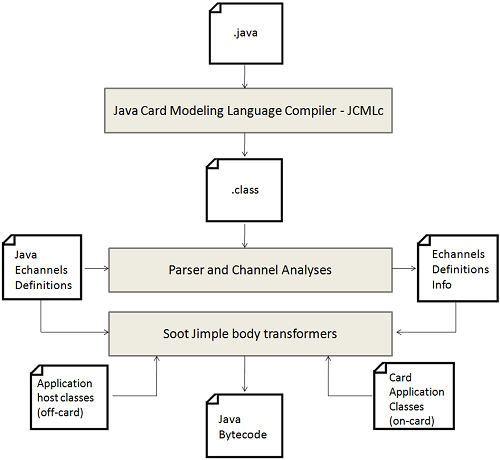
\includegraphics[width=0.45 \textwidth]{figs/SootEchannelProcess} 
\caption{High-level overview of the components of the implementation}
\label{fig:sootEchannel}   
\end{figure} 

\section{Related Works}
\label{sec:relatedWorks}

There are a few approaches that try to handle contract violation by means of
improving the exception handling behavior. The Krakatoa tool \cite{Krakatoa} for
certification of java and Java Card programs translate the java program,
annotated with JML, into the WHY \cite{FilliatreM07} input language. The WHY input language
is an ML-like minimal language, with very limited imperative features, such as
references and exceptions. On the other hand, \cite{Rebelo} defines a set of types of
faults that can happen on the interplay between java exception handling
mechanism and runtime assertions checkers (RACs) for JML. It presents an error
recovery technique for RACs that tackles such limitations. The proposed approach
uses of aspect-orientation to monitor the exceptions that represent contract
violations and force such exceptions to be signaled, preventing exceptional
handling contexts from negatively affecting RAC generated exceptions.   

The EJCFlow implementation has three advantages in terms of the aforementioned
related works. First, EJCFlow abstractions allow the explicit representations of
properties governing global exception behaviors. As a consequence, the
separation between normal and exceptional behavior is preserved, resulting in
untangled software artefacts, reusable handlers, and improved maintainability.
Second, EJCFlow abstractions make it possible to understand the potential paths
of global exceptions from an end-to-end perspective by looking at a single part
of the program. Third, EJCFlow improves reliability in evolving software by
enforcing that harmful exceptional behaviors are not added between the two ends
of a given explicit exception channel. Also, the EFlow model allows to verify
whether or not all exceptions flowing through an explicit exception channels are
correctly handled at pluggable handlers.          

 
    

\section{Conclusion} 
\label{sec:conclusion}

This paper has presented an implementation of the EFlow model whose main purpose
is to improve the exception handling mechanisms of Java Card Applications. We
leverage the JCML specification-level annotations to promote improved separation
between normal and error handling code, while keeping track of exception control
flows. Our ongoing work encompasses the empirical evaluation of the error
proneness on the use of EJCFlow when compared to conventional proposals
discussed in this paper.       

% conference papers do not normally have an appendix




% trigger a \newpage just before the given reference
% number - used to balance the columns on the last page
% adjust value as needed - may need to be readjusted if
% the document is modified later
%\IEEEtriggeratref{8}
% The "triggered" command can be changed if desired:
%\IEEEtriggercmd{\enlargethispage{-5in}}

% Better way for balancing the last page:

\balance

% references section

% can use a bibliography generated by BibTeX as a .bbl file
% BibTeX documentation can be easily obtained at:
% http://www.ctan.org/tex-archive/biblio/bibtex/contrib/doc/
% The IEEEtran BibTeX style support page is at:
% http://www.michaelshell.org/tex/ieeetran/bibtex/
%\bibliographystyle{IEEEtran}
% argument is your BibTeX string definitions and bibliography database(s)
%\bibliography{IEEEabrv,../bib/paper}
%
% <OR> manually copy in the resultant .bbl file
% set second argument of \begin to the number of references
% (used to reserve space for the reference number labels box)
\bibliographystyle{plain}
\bibliography{weh'12} 





% that's all folks
\end{document}


